\graphicspath{{../03Mathematics/pics/}}

\chapter{Mathematics}\label{ch:Mathematics}

\lettrine[lines=2]{\color{darkocre}M}{athematical concepts and tools used in quantum theory are} not significantly different from the ones used in classical physics.

\begin{myprereq}{Prerequisite Knowledge}
	To fully understand the material of this chapter, readers should be comfortable with the following concepts:
	
	\begin{itemize}
		\item \phantom{phantom}
		\vspace{-0.5cm}
		\item State
		\item Dynamical equations
	\end{itemize}	
\end{myprereq}



\section{Functions}

The idea of a function is a very basic one. Essentially, function is an unambiguous \emph{rule}, an \emph{algorithm}, which associates a certain value $y$ (\emph{result} or \emph{output} of a function) with every meaningful \emph{input} value $x$ (\emph{argument} of a function). As an example, consider the following  function:
\[
y=\frac{1}{2x^2+5}\,.
\]
For any real number $x$ we can compute the value $y$ using only basic arithmetic operations. 

Next consider a function $\btc{sqrt}$ which computes a square root of a number: $y=\btc{sqrt}\,x$. If we only work with real numbers, the range of meaningful inputs is reduced -- only non-negative input values $x$ are allowed. Another thing to notice is that now the function is simply given a name  $\btc{sqrt}$  and shows no structure -- it is not expressed in terms of other more basic operations. A few important functions are given names: 
$\sin\,,\cos\,,\exp\,,\log\,,\btc{abs}$\footnote{Absolute value of a number -- its positive magnitude.} and several more. Of course, the square root of a number is traditionally written with a special sign -- called a \emph{surd}: $\btc{sqrt}\,x=\sqrt{x}$.

\subsection{Function Boxes}
The input-output view of functions leads to a helpful picture where a given function is represented as a box with an input and an output (or multiple inputs and even multiple outputs), as illustrated in Figure \ref{fig:functionAsBox}.
\begin{figure}[htbp]
	\centering
	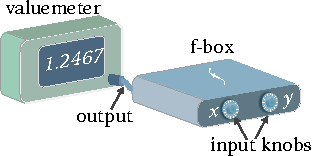
\includegraphics[scale=1.0]{functionAsBox}
	\caption{A function can be viewed as a box with input(s) and output(s).}
	\label{fig:functionAsBox}
\end{figure}


\begin{figure}[htbp]
	\centering
	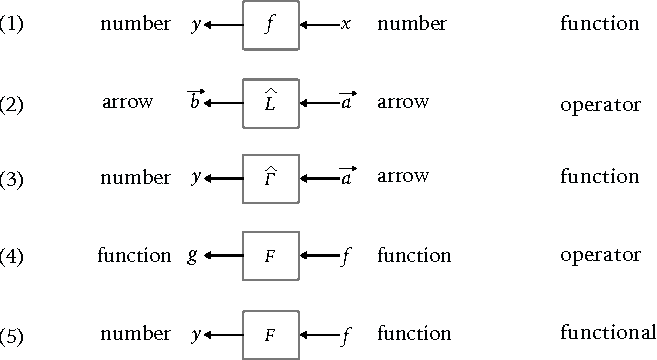
\includegraphics[scale=1.0]{functionTypes}
	\caption{Several types of functions: (1); (2); (3); (4); (5).}
	\label{fig:functionTypes}
\end{figure}

\subsection{Application Notation}
The dominant rule for writing function $f$ applied to an argument $x$ uses parentheses around the argument, like so: $f(x)$. This rule, howevers, is \emph{not absolute} and is abandoned as soon as one uses functions in linear algebra. For example, when an operator $\op{f}$ is applied to a vector $\ket{x}$, we would write $\op{f}\,\ket{x}$, without the parentheses. 

In this book we will use a uniform rule for function application: \emph{Function and its argument are separated by a space. Only structured arguments are surrounded by parentheses. Simple arguments are written without parentheses.} Thus, we will always write
\[
\sin\,x\,,\quad \exp\, x\,,\quad \textrm{abs}\,x\,, 
\]
and so on. We can even write -- without any confusion -- expressions like
\[
\cos\frac{\phi}{3}\,,\quad\log\sqrt{y}\,.
\]
However, we will always use parentheses in the expressions similar to
\[
	\tan (\alpha+\beta)\,,
\]
to avoid confusion with another valid expression: $\tan \alpha+\beta=(\tan \alpha)+\beta$.

\subsection{Multi-Input Functions}
Function of a single argument are the most familiar kind. However, functions with two inputs are also widely used. The simplest example is the function of two arguments (\emph{binary function}):
\[
\btc{add}\,x\,y = x + y\,.
\]
On the left-hand side the function is written using so-called \emph{prefix notation}, where the name precedes the arguments. On the right-hand side the same function is written using a more conventional \emph{infix notation}, in which a special symbol is placed between two arguments. Other examples if binary functions can be given:
\[
\btc{mul}\,x\,y = x * y=xy\,,
\]
\[
\btc{pow}\,x\,n = x^\wedge n =x^n\,,
\]
\[
\btc{max}\,x\,y = x\,\textrm{if}\,x>y,\,\textrm{otherwise}\,y\,.
\]
Note that the infix notation works only for binary functions and special symbols (like "$+$") exist only for small number of them. In short, infix notation, although convenient, lacks generality needed for more powerful and abstract mathematics.

Any formula expressing a physical quantity can be viewed as a function with multiple inputs. Consider Newton's law for gravitational attraction between two point-like bodies. The force is given by
\[
F = G\frac{Mm}{r^2}\,.
\]
Assuming that the gravitational constant $G$ is a fixed number, the expression for the force depends on three arguments -- two masses and the distance between them. 
\begin{exercise}
	Consider a \emph{ternary function} (function of three arguments):
	\[
	f\,M\,m\,r=Mm/r^2\,.
	\]
	Express it purely in terms of the binary function \btc{mul} and the unary function \btc{inv}.
	\label{exe:ternaryFunction}
\end{exercise}

\subsection{Partial Application}
The box-view of functions leads to a simple, yet powerful, concept of a \emph{partially applied} function. A function of multiple arguments is called partially applied if not all its "inputs" are "filled" (i.e. assigned fixed values). 

Consider, for instance, the ternary function from the Exercsie \ref{exe:ternaryFunction}. Suppose we study how two specific bodies,with masses $M=10$ and $m=1$, interact gravitationally . Then the force $F$ between these bodies is a unary function $F_r$ of the distance $r$:
\[
F_r = G*(f\,10\,1\,r) = 10G/r^2\,.
\]
Here we partially applied the ternary function $f$ to only two arguments, leaving the third argument $r$ a free parameter. As the result of such partial application we obtained a unary function of the distance $r$ between two boides.

Let's consider another example of partial application. This illustration might seem trivial, but it will help understand the role of partial application in the case of \emph{dual} objects, such as ket and bra vectors of quantum theory. First, we write a product of two numbers using prefix notation: $\btc{mul}\,x\,y$. Then, partially apply the binary function \btc{mul} to some number, say $3$. This results in a unary function \btc{trp} which simply triples the value of its argument:
\[
f_y = \btc{trp}\,y=3y\,.
\] 

\subsection{Linearity}
Some functions are simpler than others. For example, a \emph{symmetric} function has the same value for $x$ and $-x$: $f\,x=f\,(-x)$. A general function does not have such a property, and in this sense symmetric functions are simpler than a general function.

Among the simplest kinds of functions, \emph{linear functions} are of special importance. Such functions have the following properties:
\[
f\,(x+y) = (f\, x)+(f\,y)\quad\textrm{and}\quad f\,(ax)=a(f\, x)\,.
\]
These requirements are called \emph{linearity conditions}.

\begin{exercise}
	Check whether the function \btc{trp} is a linear function.
\end{exercise}

For numeric functions, the linearity conditions are very restricting. Linear numeric functions all have the same form:
\[
f_a\,x=a*x\,,
\]
for some number $a$. Thus, for each number $a$ there corresponds a linear numeric function $f_a$ and its action on any argument $x$ is a simple multiplication by the number $a$.

The simuation becomes less trivial when we consider linear functions whose arguments are not simple numbers (e.g. vectors, operators, or even functions).


\section{Numberlikes}
Physics without numbers is unimaginable. But simple numbers, like \emph{natural numbers} 1, 2, 3, and so on are very limiting.  As the range of application of mathematics increased, numbers evolved from natural numbers, to \emph{whole} numbers, to \emph{fractions}, to \emph{real} numbers, and then to \emph{complex} numbers and to \emph{quaternions}\footnote{Octanions are not used in physics widely enough to be discussed here.}. The concept of a number became increasingly less intuitive, more abstract and powerful.

Today mathematics offers several \emph{mathematical objects} which behave essentially like numbers, but which also allow more powerful manipulations and thus can be used in wider range of problems. Examples of such \emph{numberlikes} are \emph{vectors}, \emph{tensors}, and \emph{operators}. We will explore all these objects in this chapter and will see that these three concepts are actually closely related to each other (e.g. vectors are tensors, and tensors are operators!)


\begin{flushleft}
	{\it Addition}
\end{flushleft}
The essential characteristic of numbers is the ability to \emph{add} two of them to get another number:
\[
x\,\boxplus\, y = z\,.
\]
The addition operation satisfies two simple requirements
\[
x\,\boxplus\, y = y\,\boxplus\, x\quad\textrm{ -- commutativity}\,,
\]
and
\[
(x\,\boxplus\, y)\,\boxplus\, z = x\,\boxplus\, (y\,\boxplus\, z) \quad\textrm{ -- associativity}\,.
\]


Additivity is "contagious" -- it propagates to other mathematical objects which operate on "usual" numbers. For example, it is easy to give a constructive meaning to the following expression:
\[
f = \sin\boxplus\exp\,.
\]
Here we add two numeric functions to create a new function $f$. To describe this function we must specify what it does to all possible arguments. In this case it is simply
\[
f\,x=(\sin\, x)+(\exp\, x)\,.
\]
Thus, the ability to add numbers leads to the ability to \emph{add functions}. It must be emphasized, that in the expressions like $\sin\boxplus\exp$ we are not adding numerical values of the functions, we are adding functions -- completely different mathematical objects. Adding functions becomes very useful for certain function types called \emph{operators}, as explained in section \ref{sec:operators}.

\begin{flushleft}
	{\it Multiplication}
\end{flushleft}
Repeated addition of numbers leads to the idea of multiplication. For "normal" numbers mutiplication has two properties analogous to addition:
\[
x\,*\, y = y\,*\, x\quad\textrm{ -- commutativity}\,,
\]
and
\[
(x\,*\, y)\,*\, z = x\,*\, (y\,*\, z) \quad\textrm{ -- associativity}\,.
\]
Furthermore, mutiplication and addition possess \emph{distributivity}:
\[
x\,*\, (y\,+\,z)=x\,*\, y\,+x\,*\, z\,.
\]

The ability to add "normal" numbers allows one to introduce \emph{multiplication of functions}. Indeed, we can give a constructive meaning to an expression 
\[
f = \sin\boxtimes\exp\,.
\]
It must be emphasized again: this is not a multiplication of the numeric values of the functions $\sin$ and $\exp$, it is the mutliplication of the functions themselves. 
To find the value of a unary function $f$, we simply write
\[
f\,x=(\sin\,x)*(\exp\,x)=y\,*\, z\,.
\]
Now on both sides of this equality we have "normal" numbers: On the left-hand side we have the value $f\,x$ of a unary function $f$ applied to the numeric argument $x$, on the right-hand side we have to numeric values $y=\sin\,x$ and $z=\exp\,x$ multiplied in a "usual" way.

The example given above can be generalized to an arbitrary pair of unary numeric functions $f$ and $h$. It is not difficult to convince yourself that the "product" $f\,\boxtimes\, h$ is commutative, associative, and is also distributive with respect to the "addition":
\[
f\,\boxtimes\, (h\,\boxplus\, g) = (f\,\boxtimes\, h)\,\boxplus\,(f\,\boxtimes\, g)
\]
for three unary numeric functions $f$, $h$, and $g$. In other words, unary numeric functions can be made to behave like numbers. One can view functions and manipulate them as objects on their own, without referring to their arguments.
\begin{mybio}{Point-free Notation}
	Manipulating functions without explicitely writing their arguments is known as \emph{argument-free notation} or \emph{point-free notation}. It is a useful practice and is common in quantum theory.
\end{mybio}

\begin{flushleft}
	{\it Composition}
\end{flushleft}
Functions, and their "brothers" operators, allow an additional way to combine two function in order to create another one. It is called \emph{composition} or, sometimes, \emph{sequencing} of two functions. Let's illustrate the idea using the familiar functions $\sin$ and $\exp$. We can "create" (define) a function 
$f$ which acts on its input argument in the following way:
\[
f\,x=\sin\,(\exp\, x)\,.
\]
We first apply the function $\exp$ to the input argument $x$ to obtain a numeric value $y=\exp\, x$, and then apply the function $\sin$ to $y$. We applied two functions in sequence. A special notation exists for composition. We write $f = \sin\circ\exp$.

Unlike addition and multiplication, \emph{composition is not commutative}:
\[
\sin\circ\exp\ne\exp\circ\sin\quad\textrm{because}\quad\sin\,(\exp\, x) \ne \exp\,(\sin\, x)\,.
\]
However, \emph{composition is associative.} Given three functions $f$, $h$, and $g$ we can combined them in two different orders, specified by the parentheses:
\[
(f\circ h)\circ g = f\circ(h\circ g)\,.
\]
Both sides of this equality represent the same value $f\,(h\, (g\, x))$: We first evaluate $y=g\, x$, then feed it into $h$ to find $z=h\,y$, and finally input it as the argument to $f$.

\begin{exercise}
	Check whether composition is distributive with respect to an "addition" of functions.
\end{exercise}

\begin{mybio}{Composition In Quantum Physics}
	Composition is an extremely powerful way to combine functions. Composition has special significance for \emph{linear operators} -- linear functions operating on non-numeric arguments (e.g. on vectors). 
	
	In quantum theory different operators represent different measurement operations, such as  measurement of position, momentum, energy, angular momentum, spin, and so on. Only \emph{linear operators} are used in quantum theory. These operators act on special vectors.
	
	Like any two functions, two quantum operators $\op{A}$ and $\op{B}$ can be composed:
	\[
	\op{C} = \op{A}\circ\op{B}\,.
	\]
	It is customary to drop the infix composition sign and simply write $\op{C} = \op{A}\op{B}$.
	
	An operator can be composed with itself. In this case a special notation exists to avoid long and clumsy expressions:
	\[
		\op{A}\circ\op{A}=\op{A}\op{A}=\op{A}^2\,.
	\]
	In general, the expression $\op{A}^n$ represents the operator $\op{A}$ composed with itself $n$ times.
	
\end{mybio}

\section{Kalcoolus}

To arrive at the idea of vectors we will start with simple geometrical
objects -- arrows in a plane, as illustrated in the Figure \ref{fig:arrowsSpace}.

\subsection{$\Delta-\delta-\partial$ Notation}

\subsection{Bernouli Sums}

\section{Arrows}

To arrive at the idea of vectors we will start with simple geometrical
objects -- arrows in a plane, as illustrated in the Figure \ref{fig:arrowsAndVectors}.

\begin{figure}[htbp]
  \centering
  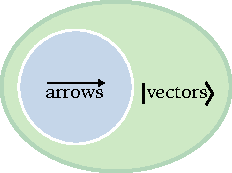
\includegraphics[scale=1.0]{arrowsAndVectors}
  \caption{Arrows provide a simple geometric example of vector quantities. The idea of vectors, however, is more powerful and extends beyond this simple representation as directed line segments.}
  \label{fig:arrowsAndVectors}
\end{figure}

Symbolically, we will denote vectors by placing an arrow over letters:
\[
\vec{a}\,,\vec{b}\,,\vec{c}\,,\ldots\,,\vec{\alpha}\,,\vec{\beta}\,.
\]

\subsection{Dirac Notation}

\section{Scalar Product}

To arrive at the idea of vectors we will start with simple geometrical
objects -- arrows in a plane, as illustrated in the Figure \ref{fig:arrowsSpace}.


\section{Operators}\label{sec:operators}

To arrive at the idea of vectors we will start with simple geometrical
objects -- arrows in a plane.
\[
\braket{\phi}{\phi}
\]
and
\[
\ketbra{\phi}{\phi}\,.
\]
\begin{example}
	Consider an operator that transforms the state $\ket{0}$ into a linear combination $\ket{+}=(\ket{0}+\ket{1})/\sqrt{2})$ and the state $\ket{1}$ into a linear combination $\ket{-}=(\ket{0}-\ket{1})/\sqrt{2})$.
	
	It is called \emph{Hadamard} operator and has the following matrix representation.
\end{example}

\subsection{Super-operators}

An action of an operator $F$ on arrows can be represented symbolically
as an equation:
\[
F\,\vec{a}=\vec{b}\:.
\]
Often a ``hat'' is placed on top of an operator\footnote{In Quantum
	Mechanics, for example.}, to emphasize that it is different from
numeric function:
\[
\colorboxed{red}{
	\op{F}\,\vec{a}=\vec{b}\:.
}
\]

\begin{mybio}{Simple Operators}\\
	It is easy to come up with examples of operators:
	
	\begin{itemize}
		\item\phantom{x}
		
		\item Unit operator (or \emph{identity} operator), such that
		\[
		\op{I}\,\vec{a}=\vec{a}\,.
		\]
		
		\item ``Zeroing'' operator that maps every vector into a zero
		vector:
		\[
		\op{0}\, \vec{a} = \vec{0}\,.
		\]
		
	\end{itemize}
\end{mybio}


To fully describe an operator, we must describe how it acts \emph{on
	every} arrow. 

\begin{flushleft}
	{\bf Examples}
\end{flushleft}
Let us take a closer look at a couple of operators. While studying
these examples we must keep in mind that the relations between
components are \emph{specific to basis} and will change if we change the
basis. The question of how exactly the relation between components
changes will be addressed later in Section
\ref{sec:ComponentTransformation} for the simplest types of operators.


\begin{mybio}{Matrix}
	Here is an example of matrix:
	\[
	\op{S} =
	\begin{pmatrix}
		S_{11} & S_{12}\\
		S_{21} & S_{22}
	\end{pmatrix} =
	\begin{pmatrix}
		\alpha & 0\\
		0 & \alpha
	\end{pmatrix}\,.
	\]
	Similar approach can be used to find the components of any linear operator.
\end{mybio}


\section{Functionals}
Another important type of function is called \emph{functional}. A functional maps a function into a number. Let's consider several examples.

\begin{flushleft}
	{\it Total Mass}
\end{flushleft}
Suppose an astrophysicist is trying to model a spherically symmetric star and calculates \emph{density} of the star as the function of distance from its center: $r\rightarrow\rho_r$. The total mass of the star can then be evaluated as the sum of masses of all spherical shells with thickness $\delta r$:
\[
M = \int \delta V\rho_r=\int 4\pi r^2\delta r\rho_r\,.
\]
For a given function $\rho_r$ this summation will result in a number -- star's total mass. Such mapping $\rho_r\rightarrow M$ is an example of a functional.

\begin{flushleft}
	{\it Total Fuel}
\end{flushleft}
Consider a car moving on a straight highway between two points $A$ and $B$. The amount of fuel the engine consumes at a given moment depends on the speed of the car at that moment and can be described by the function $\mu_v$. Suppose the position of the car as the function of time $x_t$ is known and are looking for the total fuel consumed during the travel. This can be done in three steps. 

First, we find the speed of the car as the function of time by applying the operator $\partial_t$ to $x_t$: $v_t=\partial_{t}x$. Second, we find the fuel consuption rate $\mu$  as the function of time by plugging $v_t$ into $\mu_v$: $f_t = \mu(v_t)$. Finally, we can find the total amount of consumed fuel as the sum
\[
F = \int f_t\delta t\,.
\]
Combining all three steps into a single mathematical expression will result in a more cumbersome formula:
\[
F = \int \delta t\mu(\partial_t x)\,.
\]
This formula encodes a recipe for mapping any function $x_t$ into a number $F$ -- an example of a functional.

\begin{flushleft}
	{\it Total Action}
\end{flushleft}
A body in a "free fall" is moving with constant acceleration due to the force of gravity. Its speed increases as the body approaches the ground. If the body starts at rest at height $H$, its position along the vertical $y$ axis depends on time as $y_t=H-gt^2/2$ and the velocity changes according to the equation $v=-gt$.

The potenital energy $E_p=mgy$ of the body decreases, while its kinetic energy $E_k=mv^2/2$ grows. The total mechanical energy $E=E_p+E_k$ remains fixed according to the law of energy conservation. Thus, the potential energy of the body is transformed into the kinetic energy.

Another physical quantity is often important -- the \emph{imbalance} of kinetic energy over the potential energy:
\[
L = E_k - E_p\,.
\]
It does not remain constant, and for the case of a free fall we can easily find its time dependence:
\[
L_t = mg^2t^2 - mgH\,.
\]
Given $L_t$, we can calculate a fundamental physical quantity -- total \emph{action} of the process:
\[
A = \int\delta t L_t\,.
\]
The summation extends to the moment $t=T$ when the body reaches the ground ($y=0$). This happens at $T=\sqrt{2H/g}$.

Performing the summation requires evaluation of two familiar sums:
\[
\int t^2\delta t =\frac{T^3}{3}\quad\textrm{ and }\quad \int \delta t=T\,.
\]
Substituting the values of $T$ and simplifying, the expression for the total action takes the form
\[
A = mgT(\frac{gT^2}{3}-H)=-\frac{mH}{3}\sqrt{2gH}=-\frac{mv_{m}H}{3}\,.
\]
Here we used $v_m=gT=\sqrt{2Hg}$ -- the maximal speed of the body at the end of the free fall process. Finally, denoting the maximum momentum of the body as $p_m=mv_m$, we obtain $A=-p_m H/3$. Note that the action can be expressed as the product of momentum and distance.

\emph{Action} is a physical quantit of fundamental importance. It plays a prominent role in both classical mechanics (the principle of \emph{stationary action}) and in quantum physics (the principle of \emph{action quantization}). Both principles will be explored in details later in the book.

\begin{exercise}
	Calculate the total action of a free fall process for an electron falling from the height 0.1 meter.
\end{exercise}


\begin{flushleft}
	{\it Assorted Examples}
\end{flushleft}
Examples of functionals given above involve evaluation of sums in order to find  \emph{total quantities} of various kinds:
\[
Q = \int \delta x f_x\,.
\]
The total quantity $Q$ depends on the behavior of the input function $f_x$ over an extended range of $x$ values. Simpler forms of functionals can also be used. For example:
\[
\mathcal{M}\, f = f_0
\]
returns the value of the input function $f_x$ at zero. This functional, despite its trivial look, is very useful and widely used in physics and mathematics. Its rigorous mathematical form is called \emph{Dirac delta function}\,.
\begin{mybio}{Dirac Delta Function}
	The idea of delta function is simple: it describes the density of mass (or charge, probability, and so on) for a point-like particle. Formally, such density can be written as $\delta_x$.
	
	Since the total mass (charge, probability) is finite, the summation of the density over the region where the particle might be must be a fixed number:
	\[
	m = \int \delta x \delta_x\,.
	\]
\end{mybio}

Another example of a simple functional is the maximum of a function:
\[
\mathcal{X}\,f = \textrm{max}\,f_x\,.
\]
Finally, one can map any function $f_x$ into a number like so:
\[
\mathcal{R}\,f = \frac{f_1}{1!} + \frac{f_{1/2}}{2!} + \frac{f_{1/3}}{3!}+\ldots+\frac{f_{1/n}}{n!}+\ldots\,.
\]
For $f=\sin$ we obtain $\mathcal{R}\,\sin\approx 1.1479$.
\begin{exercise}
	For the functionals $\mathcal{M}$, $\mathcal{X}$, and $\mathcal{R}$ check whether they are \emph{linear}.
\end{exercise}

\section{Spaces}

To arrive at the idea of vectors we will start with simple geometrical
objects -- arrows in a plane.
\[
\braket{\phi}{\phi}
\]
and
\[
\ketbra{\phi}{\phi}\,.
\]

\section{Duality}

To arrive at the idea of vectors we will start with simple geometrical
objects -- arrows in a plane.
\[
\braket{\phi}{\phi}
\]
and
\[
\ketbra{\phi}{\phi}\,.
\]


\section{Bundling}
A pair of vectors can be combined in a variety of ways. For example, adding two vectors returns the third vector, while scalar product returns a number. Other useful methods of combining vectors result in more advanced mathematical objects, such as, for example, tensors. One simple approach to combining vectors to create complex objects uses the idea of \emph{bundling}.

When a pair of vectors is bundled, the original vectors are not lost, they become incorporated in a more complex mathematical object. It may sound complicated, but the idea can be expressed simply as follows: \emph{Keep original vectors together in some some sort of a bundle.}

The simpest bundle is a pair. Given two vectors of the same type $\ket{a}$ and $\ket{b}$ we can bundle them into a pair: $\mathcal{P}=(\ket{a}, \ket{b})$.

\[
\ketbra{a}{b}\,.
\]
\begin{exercise}
	Write Hadamard operator in terms of the tensor product of vectors $\ket{0}$, $\ket{1}$, $\ket{+}$ and $\ket{-}$.
	
	\[
	\op{H} = \ketbra{+}{0}+\ketbra{-}{1}\,.
	\]
\end{exercise}

\section{Functions As Vectors}

To arrive at the idea of vectors we will start with simple geometrical
objects -- arrows in a plane.
\[
\braket{\phi}{\phi}
\]
and
\[
\ketbra{\phi}{\phi}\,.
\]

\section{Application: Circular Motion}
Let us examine how the concepts and tools discussed above can be applied to a simple case of circular motion.  

Consider a  particle moving in a circle with the radius $R$, as shown in Figure X. If we choose the center of the circle as the reference point, we can specify the position of the particle using an arrow $\ket{r}$. During motion the direction of this arrow is constantly changing, but its length $R$ remains the same.  

After a short time interval $\delta t$, the position of the particle changes by $\delta\ket{r}$:
\[
\ket{r_t}\quad\rightarrow\quad \ket{r_{t+\delta t}} = \ket{r_t}+\delta\ket{r}\,.
\]

The length of the path covered by the particle during the time interval $\delta t$ can be approximated by the length of the arc  $\delta L=R\delta\theta=v\delta t$. The arrow $\delta\ket{r}$ can be written as $\delta L\ket{u}$ where $\ket{u}$ is the vector of unit length pointing in the direction of motion. This unit vector can be constructed from $\ket{r}$ by scaling it down by $R$ and then rotating counter-clockwise with the operator $\op{J}$: 
\[
\delta\ket{r}=R\delta\theta\op{J}\left(\frac{\ket{r}}{R}\right)\,.
\]
Since $\op{J}$ is a linear operator, the $R$ cancels and we can write
\[
\frac{\delta\ket{r}}{\delta t}=\frac{\delta\theta}{\delta t}\op{J}\ket{r}\qquad\Longrightarrow\qquad
\partial_t\ket{r}=\omega\op{J}\ket{r}\,,
\]
where we introduced the angular speed $\omega=\partial_t\theta$. Finally, by applying the $\op{J}$ operator to both sides of the last equation, we can cast it into the "Schrodinger" form:
\[
\op{J}\partial_t\ket{r}=-\omega\ket{r}\,.
\]  



\section*{Chapter Highlights}
{\setstretch{1.5}\chhc
  \it
\begin{itemize}
\item Arrows in a plane provide a simple model for vectors.
\item Arrows can be manipulated in ways analogous to numbers: Two arrows
  be added, an arrow can be ``scaled'' (stretched or compressed). Arrows form
  an algebra.
\item Basis is an extremely important concept. Basis is a set of
  objects (arrows) that can be used to ``build'' all other similar
  objects (arrows). At the same time, basis can not be used to build
  itself -- basis arrows are independent.
\end{itemize}
}
